\section{SLAM}

Simultaneous Localization And Mapping (SLAM)\cite{FirstSLAMMention}\cite{SLAMIntro} refers to both the problem and the algorithms that tries to solve it. The problem is to incrementally build a map of landmark observations, while also locating the agent which observes these measurements in the map. Popular solutions to this include EKF-SLAM\cite{EKFSLAM}, FastSLAM\cite{FastSLAM1} and factor graph\cite{Dellaert} solutions like iSAM2\cite{iSAM2}. These solutions are explained in detail below. 

The problem is usually formulated probabilistic. The important variables used in the formulation are the following:

\begin{itemize}
    \item $x_k$: The pose of the agent at time $k$. 
    \item $u_k$: The vector of inputs that move the agent to the pose $x_k$ at time $k$.
    \item $m_i$: A vector containg the location of the $i$th landmark in the map frame. 
    \item $z_k$: A vector of all the measurements of the relative positions of landmarks that can be measured from the agent at time $k$ 
\end{itemize}

There is also a number of sets that are needed

\begin{itemize}
    \item $X_{0:k} = \{x_0,x_1,...x_k\} = \{X_{0:k-1},x_k\}$: The history of all the agents poses.
    \item $U_{1:k} = \{u_1,u_2,...,u_k\} = \{U_{1:k-1},u_k\}$: The history of all control inputs.
    \item $m=\{m_1,m_2,...,m_n\}$: The set of all landmarks, also called the map.
    \item $Z_{1:k}=\{z_1,z_2,...,z_k\} = \{Z_{1:k-1},z_k\}$: The set of all landmark observations that have been measured until time $k$.
\end{itemize}

The problem can now be formulated as computing the probability distribution 

\begin{equation}
    P(x_k,m|Z_{0:k},U_{0:k},x_0)
\end{equation}

at every time step $k$. This is the joint posterior density of location of all landmarks in the map and the agents pose, given all the measurements that have been seen so far and the control inputs that have been applied to the agent. 

One usually wants to compute this distribution reccursively. This is done by using the previously computed distribution $P(x_{k-1},m|Z_{0:k-1},U_{0,k-1},x_0)$ at the previous time step $k-1$, together with a model for the next pose of the agent given the current input and pose, 

\begin{equation}
    P(x_k|x_{k-1},u_k)
\end{equation}

and a measurement model, giving the probability of making an observation $z_k$ when both the agents pose and the landmarks location is known

\begin{equation}
    P(z_k|x_k,m)
\end{equation}

The standard way of doing it now is doing a two part update of to get the desired distribution. First a time update, that uses the motion model to find an estimate for the agents location


\begin{align}
    P(x_k,m|Z_{0:k},U_{0:k}, x_0) 
     = & \int P(x_k|x_{k-1},u_k) \\
    & \times P(k_{k-1},m|Z_{0:k-1},U_{0:k-1},x_0)dx_{k-1}
\end{align}

The second update is to include the effect of measurements, 

\begin{equation}
\begin{split}
    P(x_k,m|Z_{0:k},U_{0:k},x_0) 
    = \frac{P(z_k|x_k,m)P(x_k,m|Z_{0:k-1},U_{0:k},x_0)}{P(z_k|Z_{0:k-1},U_{0:k}}
\end{split}
\end{equation}

How the method describes the motion model and measurement model, and how it does the two updates differ from method to method, but this is the main idea that lies behind them all. The SLAM problem has been said to have been solved, but this is only meant theoretically; in practice there are still problems with all of the methods. The main challenges that are still not overcome completely are 

\begin{itemize}
    \item How to update in real time.
    \item How to build a consistent map that doesn't make the computational demand grow exponentially.
    \item How to associate measurements to landmarks.
\end{itemize}

\subsection{EKF}

One of the first solution to the SLAM problem was the EKF-SLAM\cite{EKFSLAM}. It assumes a motion model 

\begin{equation}
    P(x_k|x_{k-1},u_k) \iff  x_k = f(x_{k-1},u_k) + w_k
\end{equation}

where $f(x_{k-1},u_k)$ is the model of the vehicle kinematics and $w_k$ is additive, zero mean, uncorrelated Gaussian noice with covariance $Q_k$. The observation model is similarily assumed to be 

\begin{equation}
    P(z_k|x_{k-1},m) \iff  z(k) = h(x_{k},m) + v_k
\end{equation}

where $h$ is a function describing the geometry of the observations and $v_k$ is additive, zero mean, uncorrelated Gaussian noise with covariance $R_k$. 

Using the above models, the standard EKF can be used to compute the mean 

\begin{equation}
    \begin{bmatrix} \hat{x}_{k|k} \\ \hat{m}_k \end{bmatrix} = E[\begin{bmatrix} x_k \\ m \end{bmatrix} | Z_{0:k}]
\end{equation}

and the covariance

\begin{align}
    P_{k|k} &= \begin{bmatrix} P_{xx} & P_{xm} \\ P^T_{xm} & P_{mm} \end{bmatrix} \\
     &= E\bigg[\begin{bmatrix} x_k-\hat{x}_k \\ m - \hat{m}_k\end{bmatrix}\begin{bmatrix} x_k-\hat{x}_k \\ m - \hat{m}_k\end{bmatrix}^T \bigg| Z_{0:k} \bigg]
\end{align}

of the desired joint posterior distribution $P(x_k,m|Z_{0:k},U_{0:k},x_0)$. This is done by first time-updating using

\begin{align}
    \hat{x}_{k|k-1} &= f(\hat{x}_{k-1|k-1},u_k)
    P_{xx,k|k-1} &= \nabla f P_{xx,k-1|k-1}\nabla f^T + Q_k 
\end{align}

Here $\nabla f$ is the jacobian of f at the previous estimate $\hat{x}_{k-1|k-1}$. The landmarks aren't updated, since they are assumed stationary. The measurement update is then

\begin{align}
    \begin{bmatrix} \hat{x}_{k|k} \\ \hat{m}_k \end{bmatrix} &= 
    \begin{bmatrix} \hat{x}_{k|k-1} \\ \hat{m}_{k-1} \end{bmatrix}
    + K_k[z(k) - h(\hat{x}_{k|k-1},\hat{m}_{k-1}] \\
    P_{k|k} &= P_{k|k-1} - K_kS_kK_k^T
\end{align}

where the innovation, $S_k$, is defined as

\begin{equation}
    S_k = \nabla hP_{k|k-1}\nabla h^T + R_k
\end{equation}

and the Kalman gain, $K_k$, is defined as

\begin{equation}
    K_k = P_{k|k-1}\nabla h^T S_k^{-1}
\end{equation}

Here $\nabla h$ is the jacobian of h computed at $\hat{x}_{k|k-1}$ and $\hat{m}_{k-1}$. 

This solution to the SLAM problem has been proven to converge if the motion model and measurement model is correct. It does however suffer from a quadratically growing complexity in the number of landmarks, and will not be possible to implement in real time if the total map size gets too big. It also is very sensitive to incorrect associations between measurements and landmarks and since it is a linear approximation to the true model, it has the same problems that the EKF does in terms of divergence from the true solution. 

\subsection{FastSLAM}

Theoretically, one could use a particle filter\cite{ParticleFilter} to solve the SLAM problem. But practically, the particle filter can't deal with the high dimensionality of the state space, making it computationally unfeasible without any modifications. One such modification is the Rao-Blackwellized Particle Filter (RBPF)\cite{RBPF}. It assumes it's possible to partition the state, $\xi$, into two states, $\xi_1$ and $\xi_2$, that has a joint probability distribution 

\begin{equation}
    P(\xi_1,\xi_2) = P(\xi_2|\xi_1)P(\xi_1)
\end{equation}

where the conditional probability $P(\xi_2|\xi_1)$ is possible to represent analytically. This means that only $P(\xi_1)$ needs to be represented by sampling particles. The effect of this is that the marginal $P(\xi_2)$ is possible to compute with less particles, greatly reducing the computational complexity. 

Applying this mindset to the SLAM problem results in what is known as FastSLAM\cite{FastSLAM1}. The idea is that since the error in landmarks will all depend on the error in pose, the pose is the only variable in $\xi_1$. The remaining set of variables, $\xi_2$, is then the map, which is found by conditioning on the state and the measurements. This leads to the following factorization of the joint distribution

\begin{equation}
    P(X_{0:k},m|Z_{0:k},U_{0:k},x_0) = P(m|X_{0:k},Z_{0:k})P(X_{0:k}|Z_{0:k},x_0)
\end{equation}

Furthermore, it is assumed that the landmarks are independent of each other, i.e. that the joint landmark distribution $P(m|Z_{0:k},x_0)$ can be written as the product of each landmarks distribution

\begin{equation}
    P(m|X_{0:k},Z_{0:k}) = \prod_{1<i<n}P(m_i|X_{0:k},Z_{0:k})
\end{equation}

The method then employs $R$ particles, that each represent a pose, calculated by using a normal particle filter by propagation using a motion model, weighting using the measurement model and resampling. Each particle has a map, that is calculated analytically by the particle trajectory, measurements and the measurement model. This is the same as saying that each particle has a set of $n$ small EKFs, that each try to estimate the position of each landmark. 

The independence assumption between the landmark distributions mean that the complexity of the computations can be kept to $Rlog(n)$, compared to $n^2$ of the EKF-SLAM. 

There are two different version of FastSLAM: FastSLAM 1.0\cite{FastSLAM1} and FastSLAM 2.0\cite{FastSLAM2}. The difference lies in the proposal and weighting functions. 

FastSLAM 1.0 uses the motion model 

\begin{equation}
    x_{k,i} ~ P(x_k|x_{k-1,i},u_k)
\end{equation}

as a proposal function, which gives that the weights are calculated using the marginalized observation model

\begin{equation}
    w_{k,i} = w_{k-1,i}P(z_k|X_{0:k,i},Z_{0:k-1})
\end{equation}

For FastSLAM 2.0 however, the proposal function uses the latest observation $z_k$,

\begin{align}
    x_{k,i} &= P(x_k|X_{0:k-1,i},Z_{0:k},u_k) \\
    &= \frac{1}{C}P(z_k|x_k,X_{0:k-1,i},Z_{0:k})P(x_k|x_{k-1,i},u_k)
\end{align}

Where C is a normalizing constant. This gives that the importance weights are calculated as

\begin{equation}
    w_{k,i} = w_{k-1,i}C
\end{equation}

According to \cite{SLAMIntro} this leads to a weighting function that is locally optimal. This means that it gives the smallest posible variance in the weight $w_{k,i}$, given $X_{0:k-1,i}$, $Z_{0:k}$ and $U_{0:k}$.

\subsection{Factor graphs}

Talk about bayesian networks, how they're nice for representing the problem but unfit for doing the optimization. Talk about the graphical extension to bayesian networks that factor graphs are, how they solve the problem and how they represent all the different data. Maybe also a part about how they allow us to do optimization on only a small part of the problem at a time. 

Mention loop closures. Should there be a part about how we do loop closures?? I think so. 

Talk about how since we are doing featureless SLAM we need some sort of front end doing data association, so it transitions well into the next section about data association.

One new developement in the SLAM community is the developement of factor graph based approaches. This is by many considered state of the art, and some of the algorithms to come out of this approach tackles issues that haven't been possible to solve other ways. In the following the factor graph and some of the algorithms that uses it are explained. The subject is graphical in nature, and a few examples are therefore in place. Many of the main points of the discussion are paraphrased from Frank Dellaert's amazing book on the subject\cite{Dellaert}. \todo{Is this okay to say?}

\subsection{Bayesian network}

One very intuitive way of representing the SLAM problem is through a Bayesian network, or Bayes net for short. It's a graphical way of representing a joint probability density function that easily shows the different conditionings and relationships between variables. 

To be more precise, a Bayes net tries to model the joint pdf, $p(\theta)$, of all the random variables of interest, $\Theta = \{\theta_1, ..., \theta_n$, as a product of conditional probabilities

\begin{equation}
    p(\Theta) = \prod_j p(\theta_j|\pi_j)
\end{equation}

where $\pi_j$ is the set of variables that $\theta_j$ depends on. For the offline SLAM problem the variables of interest would be the set of poses, $X$, and set of measurements, $Z$, that the agent has been in and observed, respectively. In other words, $\Theta = \{X,Z\}$. 

This is best illustrated through an example. Let's say we have a two poses, $x_1$ and $x_2$. The first pose we have an initial guess on, $p(x_1)$, and $x_1$ is also measured. Call this measurement $z_1$, with measurement model $p(z_1|x_1)$. In addition we have a conditional probability distribution on the second pose given the first, $p(x_2|x_1)$. This is the motion model. 

In addition there are two landmarks, $m_1$ and $m_2$, with pdfs on their location $p(m_1)$ and $p(m_2)$. In the first pose the agent measured the location of $m_1$ relative to himself. Call this measurement $z_2$. It has a measurement model that depends on both the landmark and the pose of the agent, $p(z_2|x_1,m_1)$. Similarily the agent also measured $m_2$ from pose $x_1$ and from pose $x_1$. Call these measurements $z_3$ and $z_4$ respectively, with corresponding measurement models, $p(z_3|x_1,m_2)$ and $p(z_4|x_2,m_2)$. 

\begin{figure}
    \centering
    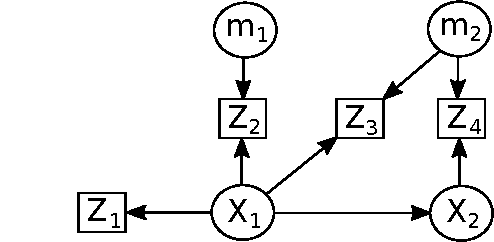
\includegraphics[width=0.8\linewidth]{0_Images/3_Background/BayesNet.pdf}
    \caption[Example of a Bayes net.]
    {Example of a Bayes net, used for a simple SLAM problem. The $x_i$'s represent poses, $z_i$'s represent measurements and $m_i$'s represent landmarks.}
    \label{Fig:BayesNet}
\end{figure}

This is represented as a Bayes net in figure \ref{Fig:BayesNet}. Here the arrows imply that the variable being pointed to depends on the variable the arrow points away from. This way all the conditional probabilities are easy to see. The Bayes net leads to the following factorization of the joint distribution

\begin{align}
    p(X,Z) = \; & p(x_1)p(x_2|x_1) \\
    \times \; &p(m_1)p(m_2) \nonumber \\
    \times \; &p(z_1|x_1) \nonumber \\
    \times \; &p(z_2|x_1,m_1) \nonumber \\ 
    \times \; &p(z_3|x_1,m_2)p(z_4|x_2,m_2) \nonumber 
\end{align}

In a SLAM setting one usually don't have any priors on the map or the pose, so $p(x_1)$, $p(m_1)$ and $p(m_2)$ are dropped. 

The 